%!TEX root = main.tex


\section{Implementation and Usage}

With explicit managed state and a pipelined snapshotting algorithm at its core, Flink maintains a rich ecosystem of backends, connectors and other services that interplay seamlessly and enrich further the capabilities of its global state establishment mechanism. In this section we summarize how each of these subsystems builds on-top of Flink's core architecture, while expanding it with asynchronous communication, delivery guarantees and external state querying support.

\label{sec:implementation}

\subsection{State Backend Support}

Managed state consistency is coordinated by Flink's snapshotting algorithm (\autoref{sec:snapshots}), however, state access and persistence are the main concerns of the state backend module. There are currently three different backends supported by the Flink stack : 1) \emph{In-Memory}, 2) \emph{File-Based} and 3) \emph{Out-of-Core}. Depending on the overall expected managed state accumulated in a pipeline, each of the backends offers a suitable trade-off between execution throughput, scalability and flexibility.

\para{In-Memory}
The \emph{In-Memory} backend maintains active managed state in local, allocated heap space and snapshotted state within the Job Manager's heap space. This is, in some distinct use-cases, a preferable choice that yields very high throughput. For example, pipeline testing and debugging or actual deployments with low state capacity requirements such as filtering and basic ETL can make a reasonable use of this backend. Upon each task's \texttt{triggerSnapshot()} invocation local state is serialized, copied and transfered to the Job Manager together with typical snapshot metadata. As a result, the Job Manager needs to have enough heap space allocated in order to be able sustain all physical task materialized states for each snapshot.

\para{File-Based:}
In most cases, complete pipeline snapshots involve much larger active managed state than what can fit in memory of a single node. The \emph{File-Based} backend leaves distributed uncommitted state in heap space, however, whenever snapshotting is invoked the state is being copied from heap to a configured distributed file system directory (e.g., HDFS). As a result, snapshot metadata is also kept to a minimum (containing mainly file references), while throughput can remain high since operations on uncommitted memory happen in-place at the local heap.

\para{Out-of-Core:}
Complex pipelines often need to maintain very large managed state such as Terabytes of indexes and large sequences of sliding windows upon which user-defined logic can operate continuously. In such cases, local heap space is insufficient to maintain even locally accessed active state, especially for certain task operators (e.g., Flink's \texttt{WindowOperator}). Flink provides an \emph{out-of-core} backend that decouples state operations performed on each task from the physical location where state itself is persisted and updated. In its current implementation, out-of-core state is interfaced with an embedded file-backed key-value database (i.e., RocksDB). Therefore, state capacity is only limited by the file system space allocated at the host where this backend is deployed. Moreover, operations triggered on managed state such as \texttt{update} for mutable state and \texttt{add} for append-only \texttt{ListState} are carried over to the embedded key-value store instead. One of the benefits that are enabled out-of-the-box with such a scheme is that most per-key operations can be executed asynchronously at the backend without sacrificing throughput. On the other hand, state value retrievals can take more time to complete, especially if some specific state has to be retrieved from compacted files on disk and it is no longer within the backend's memory. \paris{@stefan please add or correct whatever you see fit. You know this part better than anyone else.}

\subsection{Asynchronous Snapshots and Notifications}
\label{sec:async}
One of the advantages of the pipelined snapshotting protocol presented in \autoref{sec:snapshots} is that it does not restrain the actual acquisition of snapshots to be synchronous. A call of \texttt{triggerSnapshot()} by each task is expected to create an identical copy of the current state of that task. In case there is support by a backend module to execute this operation asynchronously, it can be used without violating consistency. The \emph{out-of-core} backend of Flink offers the capability to trigger snapshots in a purely asynchronous way by copying the full compacted key-value database to a backup directory by another thread, thus, letting normal processing proceed without interruptions. Once local snapshotting operations have been completed the notifications are triggered back at the tasks and carried out to the \emph{JobManager} alongside associated meta-data where a full snapshot can be declared as complete. Asynchronous snapshotting also unlocks the possibility to multiplex multiple instances of the protocol running at the same time in a dataflow graph. That means that while for example a periodic snapshot is undergoing, a user can also trigger a savepoint and both of the associated snapshots will run concurrently and distributively, each invoking its own asynchronous state copy and epoch.

Another feature that is provided to tasks as an optional asynchronous subscription-based mechanism is to trigger notifications about completed snapshots back at the tasks that request them. This is especially useful for garbage collection, discarding write ahead logs or for executing output commit protocols as we explain further in \autoref{sec:outputcommit}.

\subsection{Queryable State}
\paris{We can briefly mention how queryable state is implemented for accessing uncommitted active state from outside the system.}

\subsection{Output Commit}
\label{sec:outputcommit}

So far we have considered consistency guarantees associated with the internal state of the system. However, it is most often important to offer guarantees regarding the side effects that a pipeline leaves to the outside world, whether that is a distributed database, file system or message queue. A pipeline interfaces with the outside world mainly via its dataflow sinks. Thus, it is often crucial that sinks can offer exactly-once delivery guarantees. The feasibility of achieving ``read-committed'' isolation guarantees to external writes depends on the properties of the system upon which sinks commit output and typically comes at a higher latency cost that can, at-times, violate strong SLAs on latency. A pipeline can always be halted between snapshots after a failure or an urgent reconfiguration request and both input and state can be rolled back consistently, as it was described in \ref{sec:core}. However, the same cannot always be guaranteed about the output. If sinks are connected, for example, to a printer that instantly flushes data on paper, a rollback would possibly print the same or alternating text twice. Flink's programming model is equipped with two main types of sinks that facilitate ``read-committed'' output and build on the snapshotting mechanism: the 1) Idempotent Database Sink and 2) Bucketing File Sink.

\para{Idempotent Database Sink: } Idempotency is a property used extensively by several systems at the presence of failures in order to encourage repeatability and alleviate bookkeeping efforts and complex decision protocols to offer delivery guarantees\cite{CUSTOM:web/SparkStructuredStreaming,millwheel}. Flink's database sink executes user-defined, idempotent database queries to a distributed database for each input received per parallel sink. Deterministic streams (that do not involve stream interleaving or other forms of non-determinism) can rely on that sink to operate consistently with the database. However, in most cases where deterministic processing cannot be guaranteed, a write-ahead log of prepared query statements is kept as part of the state of that sink and maintained per-epoch. Once an asynchronous notification (\autoref{sec:async}) arrives regarding a completed epoch snapshot, the database sink commits all pending writes to the database at the expense of additional output latency (for a snapshot to complete and its notification to arrive to the sinks). Query idempotency guarantees that even failures during committing can be resolved by simply re-committing the same queries and thus, eventually, leaving the same side effects upon subsequent system reconfigurations. \paris{what are the database properties required and why is it only cassandra based?}

\begin{figure}[t!]
\centering
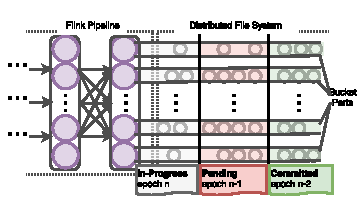
\includegraphics[width=\textwidth / 2]{figures/filecommit.pdf}
\caption{A visualization of Bucketing File Sinks.} 
\label{fig:filecommit}
\vspace{-4mm}
\end{figure}

\para{Bucketing File Sink: } Committing state to a distributed file systems (e.g. HDFS) has to be made in a coordinated way since a file has to be consistent across all its file partitions. Flink's bucketing file sink (depicted in \autoref{fig:filecommit}) eliminates the need for a write-ahead log and eagerly appends stream output within uncommitted distributed file directories which group (or ``bucket'') partition parts by time-period. After a pre-configured inactivity time-period \texttt{in-progress} directories become \texttt{pending} and are ready to be committed. The Bucketing File Sink integrates with Flink's snapshotting algorithm and associates epochs with buckets. Once a file bucket is under \texttt{pending} mode and an asynchronous notification for an associated epoch has been received, it can be moved to a \texttt{committed} state via a \texttt{rename} operation. Potential disruptions between epochs resolve into a \texttt{truncate} (Posix) operation, which is currently supported by major distributed file systems and conveniently reverses append operations. \paris{i guess the non-truncate approach is ugly. Should we write about it?}

\subsection{Asynchronous IO}
\paris{Maybe we can simply highlight how this operates and aligns with the snapshotting protocol}

\subsection{High Availability \& Reconfiguration}
\paris{This is just an implementation specific problem. We should mention how we utilized zookeeper and offer some insights about what metadata we store since it is useful for many people actually.}

	